\section{Typ-0-Sprachen und Turing-Maschinen}

\begin{frame}{Wortproblem}
	\begin{itemize}
		\item Wortproblem für Typ-0- bzw. Typ-1-Sprachen
		\begin{itemize}
			\item Wortproblem: gegeben: $w \in \Sigma^*$, Grammatik $G$; $w \in L(G)?$
			\item Entscheidbarkeit des Wortproblems $w \in L$
			\begin{itemize}
				\item $L$ heißt entscheidbar gdw. es existiert ein Algorithmus, der für jedes $w \in \Sigma^*$ nach endlich vielen Schritten hält und die Antwort "`ja"' bzw. "`nein"' liefert
				\item $L$ heißt semi-entscheidbar gdw. ex existiert ein Algorithmus, der für jedes $w \in L$ nach endlich vielen Schritten mit Antwort "`ja"' hält, für $w \notin L$ aber kein definiertes Antwortverhalten hat (z.B. gar nicht hält)
			\end{itemize}
			\item es gilt
			\begin{itemize}
				\item Das Wortproblem für Typ-1-Sprachen ist entscheidbar
				\item das Wortproblem für Typ-0-Sprachen ist semi-entscheidbar
			\end{itemize}
		\end{itemize}
		\item akzeptierender Automat für Typ-0-Sprachen: Turing-Maschine\\
		(bzw. Linear beschränkter Automat (LBA) als Spezialfall für Typ-1-Sprachen)
	\end{itemize}
\end{frame}

\begin{frame}{Exkurs: Abzählbarkeit von Mengen}
	\begin{itemize}
		\item Mächtigkeit unendlicher Mengen A, B:
		\begin{itemize}
			\item $|A|\leq |B|$ gdw. es gibt eine injektive Abbildung $f: A \rightarrow B$
			\item $|A| = |B|$ gdw. $|A|\leq |B|$ und $|B|\leq |A|$, d.h. es existiert eine bijektive Abbildung zwischen $A$ und $B$
		\end{itemize}
		\item $A$ heißt abzählbar gdw. $A$ ist endlich, oder $|A|=|\mathbb{N}|$, d.h. $A$ lässt sich bijektiv auf $\mathbb{N}$ oder eine Teilmenge von $\mathbb{N}$ abbilden
		\item Die Menge aller geordneten Paare natürlicher Zahlen $\{(n,m)\mid n, m \in \mathbb{N}\}$ ist abzählbar
		\item es gilt: sei $\Sigma$ endliches Alphabet, dann ist $\Sigma^*$ abzählbar
		\item Folgerung: die Menge aller Algorithmen (Programm = Wort über einem endlichen Alphabet (z.B. binär)) ist abzählbar
		\item Die Menge aller Sprachen über $\Sigma^*$ (d.h. $\mathcal{P}(\Sigma^*)$) ist überabzählbar
		\item Folgerung: \emph{es gibt offensichtlich unentscheidbare Sprachen}
	\end{itemize}
\end{frame}

\begin{frame}{Semi-entscheidbare und rekursiv aufzählbare Sprachen}
	\begin{itemize}
		\item es gilt: $L$ ist entscheidbar gdw. $L$ und $\overline{L}$ sind semi-entscheidbar
		\item Def: eine Sprache $L$ heißt \underline{rekursiv aufzählbar} gdw. es gibt eine berechenbare surjektive Funktion $f: \mathbb{N} \rightarrow L$, d.h. es gilt $L=\{f(1), f(2), \ldots\}$
		\item Entscheidbare Sprachen werden alternativ auch als \underline{rekursive} Sprachen bezeichnet
		\item es gilt: $L$ ist rekursiv aufzählbar gdw. $L$ ist semi-entscheidbar
		\item es gilt: $L$ rekursiv aufzählbar $\rightarrow$ $L$ abzählbar; die Umkehrung gilt nicht
		\item es gilt: die Typ-0-Sprachen sind genau die rekursiv aufzählbaren Sprachen
	\end{itemize}
\end{frame}

\begin{frame}{Nichtdeterministische Turing-Maschinen}
	\begin{itemize}
		\item TM "`Hardware"' (Basismodell 1-Band-TM):
		\begin{itemize}
			\item Speicherband (unbeschränkt, oder halbseitig beschränkt); jede Speicherzelle kann ein Zeichen aus dem Bandalphabet aufnehmen
			\item Lese-Schreib-Kopf: kann aktuelles Zeichen lesen und überschreiben; bewegt sich danach einen Schritt nach links oder rechts (L/R) oder bleibt stehen (N)
		\end{itemize}
		\item Spezifikation TM: $M=(S, \Sigma, \Gamma, \delta, s_0, \#, F)$
		\begin{itemize}
			\item [$S$:] Zustandsmenge
			\item [$\Sigma$:] Terminalalphabet
			\item[$\Gamma$:] Bandalphabet, $\Sigma \subset \Gamma$
			\item[$\delta$:] Zustandsüberführungsrelation; $\delta \subseteq S \times \Gamma \times S \times \Gamma \times \{L, R, N\}$
			\item[$s_0$:] Startzustand, $s_0 \in S$
			\item[$\#$:] Blank-Symbol (Leerzeichen), $\# \in \Gamma \setminus \Sigma$
			\item[$F$:] Menge von Endzuständen, $F \subseteq S$
		\end{itemize}
	\end{itemize}
\end{frame}

\begin{frame}{Konfigurationsübergänge, Akzeptanzverhalten}
	\begin{itemize}
		\item Konfiguration:\\
		$(s, u\underline{\alpha}v)$: Zustand $s$, Bandinhalt $u\alpha v$, Kopf unter $\alpha \in \Gamma$, $u,v \in \Gamma^*$
		\item Konfigurationsübergänge: $\alpha, \beta, \rho, \omega \in \Gamma$, $u, v \in \Gamma^*$
		\begin{itemize}
			\item $(s_1, \alpha, s_2, \beta, R) \in \delta:$\qquad $(s_1, u\rho\underline{\alpha}\omega v) \mapsto (s_2, u\rho\beta\underline{\omega}v)$
			\item $(s_1, \alpha, s_2, \beta, L) \in \delta:$\qquad $(s_1, u\rho\underline{\alpha}\omega v) \mapsto (s_2, u\underline{\rho}\beta\omega v)$
			\item $(s_1, \alpha, s_2, \beta, N) \in \delta:$\qquad $(s_1, u\rho\underline{\alpha}\omega v) \mapsto (s_2, u\rho\underline{\beta}\omega v)$
		\end{itemize}
		\item Initialisierung:\\
		Bandinhalt: $\#\#\# w\#\#\#\ldots$, Kopf unter erstem Buchstaben von $w$
		\item TM akzeptiert $w$ (als Element von $L$), gdw. es existiert eine Folge von Konfigurationsübergängen, so dass TM in einem Endzustand hält
		\begin{itemize}
			\item "`TM hält"' bedeutet: in der jeweiligen Konfiguration gibt es keinen Folgeübergang
		\end{itemize}
	\end{itemize}
\end{frame}

\begin{frame}{Varianten von TM}
	\begin{itemize}
		\item Ein-Band-TM\\
		linksbeschränktes Band; unbeschränktes Band; Mehrspur-TM: LS-Köpfe fest verbunden
		\item Mehr-Band-TM\\
		$\delta(s, \{\sigma_1, \ldots, \sigma_k\}) = (s', \{\sigma_1', \ldots, \sigma_k'\},\{r_1,\ldots,r_k\})$\\
		$\sigma_i \in \Gamma, \sigma_j' \in \Gamma, r_m \in \{L, R, N\}$, d.h. LS-Köpfe einzeln frei beweglich
		\item Alle Varianten können sich gegenseitig simulieren und sind damit gleich mächtig
		\item Bemerkung: Codierung Bandinhalt\\
		natürliche Zahl $n \rightarrow |^n$ (unäre Darstellung, "`Bierdeckelnotation"'), oder Binärdarstellung
	\end{itemize}
\end{frame}

\begin{frame}{TM: Beispiel}
	$$L=\{a^nb^n \mid n\geq 0\}$$
	\begin{align*}
		\delta = \{&(s_0, a, s_1, x, R), (s_0, x, s_0, x, R), (s_0, \#, s_f, \#, N),\\
		&(s_1, x, s_1, x, R), (s_1, a, s_1, a, R), (s_1, b, s_2, x, R),\\
		&(s_2, b, s_2, b, R), (s_2, \#, s_3, \#, L), (s_3, b, s_3, b, L),\\
		&(s_3, x, s_3, x, L), (s_3, a, s_3, a, L), (s_3, \#, s_0, \#, R)\}
	\end{align*}
	\scriptsize
	Arbeitsweise
	\begin{itemize}
		\item [$s_0$:] erstes verbliebenes $a$ wird durch Füllzeichen $x$ überschrieben
		\item [$s_1$:] erstes verbliebenes $b$ wird durch Füllzeichen $x$ überschrieben
		\item [$s_2$:] stellt sicher, dass bis zum Wortende nur $b$'s kommen
		\item [$s_3$:] zurück zum Wortanfang
		\item falls $w\in L$: am Schluss stehen nur noch $x$ auf dem Band; Übergang in akzeptierenden Zustand $s_f$
	\end{itemize}
\end{frame}

\begin{frame}{Linear beschränkte Automaten (LBA) und kontextsensitive Sprachen}
	\begin{itemize}
		\item LBA: TM, die den Bandbereich auf dem die Eingabe steht niemals verlässt (in-place)
		\item es gilt (Satz von Kuroda): die von einem (nichtdeterministischem) LBA akzeptierten Sprachen sind die kontextsensitiven Sprachen (Typ-1).\\
		Beweisidee:
		\begin{itemize}
			\item Sei $L$ Typ-1; $(u \rightarrow v) \in P, |u|\leq |v|$;\\
			LBA: ersetzt (nichtdet.) Teilwort $v$ durch Teilwort $u$; überschreitet dabei Bandbegrenzung nicht; $w$ kann dabei auf $S$ reduziert werden, falls $w \in L$
			\item sei $M$ LBA, der $L$ akzeptiert;\\
			$G$: bilde Variablen $(s, c)$ mit $c \in \Gamma$;\\
			$P$: sei z.B. $(s_1, a, s_2, b, L) \in \delta$, korrespondierende Typ-1-Regel in $P$: $c(s_1, a) \rightarrow (s_2, c)b$ für alle $c \in \Gamma$
		\end{itemize}
	\end{itemize}
\end{frame}

\begin{frame}{Turingmaschinen und Typ-0-Sprachen}
	\begin{itemize}
		\item es gilt: die durch allgemeine TM akzeptierten Sprachen sind genau die Typ-0-Sprachen\\
		Beweis analog zu kontextsensitiven Sprachen unter Verzicht auf lineare Beschränktheit des Automaten bzw. Typ-1 Bedingung für Grammatik
		\item Abgeschlossenheit
		\begin{itemize}
			\item Sowohl Typ-0-Sprachen wie auch speziell die Typ-1-Sprachen sind abgeschlossen unter Durchschnitt, Vereinigung, Konkatenation und Stern-Produkt
			\item Typ-1-Sprachen \underline{sind} abgeschlossen unter Komplement
			\item Typ-0-Sprachen \underline{sind nicht} abgeschlossen unter Komplement
		\end{itemize}
	\end{itemize}
\end{frame}

\begin{frame}{eine entscheidbare Sprache, die nicht in $L_1$ liegt}
	\begin{itemize}
		\item Worte $w \in \Sigma^*$ sind aufzählbar: $w_1, w_2, \ldots$\\
		Damit kann jedem Wort eineindeutig eine Nummer $i$ zugeordnet werden
		\item Typ-1- (wie auch Typ-0-) Grammatiken sind Worte über einem erweiterten Alphabet $\Gamma = V \cup \Sigma \cup \{\rightarrow, ;\}$ und sind ebenfalls aufzählbar: $G_1, G_2, \ldots$\\
		Damit existiert eine bijektive Abbildung $f(w_i) = G_i (= G_{w_i})$
		\item Definiere $L_D=\{w \in \Sigma^* \mid w \notin L(G_w)\}$\\
		es gilt:
		\begin{itemize}
			\item $L_D$ ist nicht Typ-1
			\item $L_D$ ist entscheidbar
		\end{itemize}
	\end{itemize}
\end{frame}

\begin{frame}{Sprachklassen: Zusammenfassung und Ausblick}
	\begin{columns}
		\column{.5\textwidth}
		\centering
		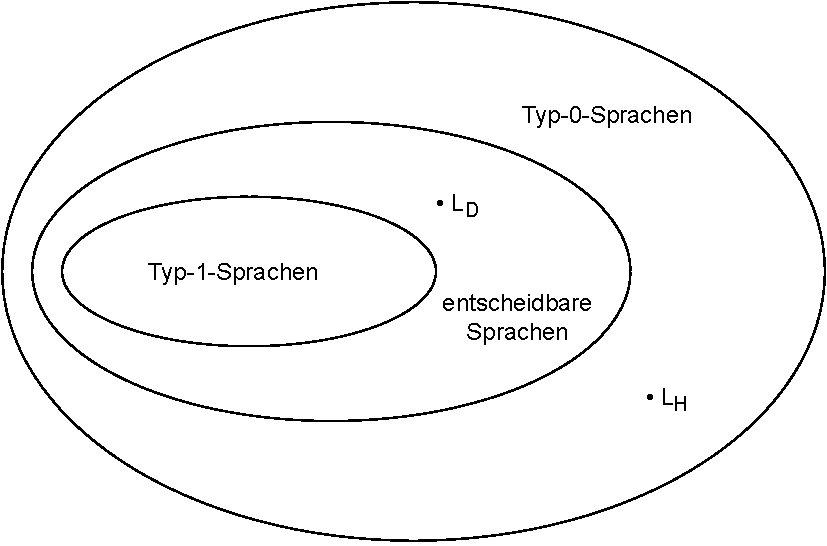
\includegraphics[width=0.9\linewidth]{images/Sprachklassen_Typ0_Typ1}
		\column{.5\textwidth}
		\begin{itemize}
			\item Typ-1-Sprachen sind entscheidbar
			\item es gibt entscheidbare Sprachen, die Typ-0 aber nicht Typ-1 sind (z.B. $L_D$)
			\item es gibt Typ-0-Sprachen, die nicht entscheidbar sind (z.B. $L_H$)
			\item es gibt Sprachen, die nicht Typ-0 sind, d.h. nicht durch eine Grammatik erzeugt werden können (z.B. $\overline{L_H}$)
		\end{itemize}
	\end{columns}
\end{frame}